\chapter{Similarity Analysis of DTM and LDA Topics}
The topics we get from both DTM and LDA are in the form of distributions. Along with the top words we also get the probability of occurrence of each word. An example of word distribution of a topic is shown in \textbf{Table \ref{table:topicDistribution}}, where the first element of the tuple is a word and the second element is the probability of this word in the current topic. We extract the top 50 words for all topics so word distribution is $K \times 50$ in LDA and $K$ is the number of topics. The top words may change in a DTM topic over time, so overall word distribution of a DTM topic varies, but it is $K \times 50 $ for one time slice, the same as an LDA topic. To check the relation between a DTM topic and an LDA topic, we use a simple but widely accepted similarity measure, the Jensen-Shannon(JS) divergence \cite{lin1991divergence}. For an LDA topic $T_{L}$ and DTM topic at time slice $t$ $T_{D}^t$, it is defined as:
\begin{equation}
JSD(T_L || T_D^t) = \frac{1}{2} D(T_L || T_{M}) + \frac{1}{2} D(T_D^t || T_{M})
 \end{equation}
 where
 \begin{equation}
  T_M = \frac{1}{2}(T_L + T_D^t)
 \end{equation}
 $D(T_L || T_{D})$ is the Kullback-Leibler divergence and can be calculated by below mentioned equation:
 \begin{equation}
D_{KL}(T_L || T_{D})  =  \sum_{w \in W} P(w| z_L) \log(\frac{P(w| z_L)}{P(w| z_D)})
 \end{equation}

 Only the top 50 words are considered for this similarity measure and word distributions do not sum up to one, so we apply normalization on both the DTM and LDA topic-word distributions.

\begin{table}[h!]
\begin{tabular}{|p{1cm}|p{13cm}|}
\hline \textbf{DTM}  &
('space', 0.0904)	('dimensional', 0.0492)	('nearest', 0.0346)	('data', 0.0341)	('projection', 0.0256)	('local', 0.0226)	('vectors', 0.0211)	('mapping', 0.0209)	('neighbor', 0.0159)	('maps', 0.0144)	('tangent', 0.0138)	('neighborhood', 0.0131)	('dimensions', 0.0125)	('dimension', 0.0122)	('dimensionality', 0.0122)	('feature', 0.0122)	('neighbors', 0.0114)	('points', 0.0097)	('kernel', 0.0091)	('point', 0.0091)	('coordinates', 0.0091)	('transformation', 0.0083)	('quantization', 0.0076)	('euclidean', 0.0074)	('projections', 0.0064)	('locally', 0.0064)	('manifold', 0.0062)	('structure', 0.0062)	('distances', 0.0059)	('reduction', 0.005)	('onto', 0.0048)	('spaces', 0.0048)	('nonlinear', 0.0044)	('topology', 0.0042)	('topological', 0.004)	('subspace', 0.004)	('directions', 0.0039)	('invariant', 0.0037)	('product', 0.0037)	('knn', 0.0036)	('coordinate', 0.0035)	('closest', 0.0034)	('matrix', 0.0031)	('mapped', 0.003)	('principal', 0.003)	('two', 0.003)	('multidimensional', 0.0029)	('laplacian', 0.0027)	('rbf', 0.0025)	('rotation', 0.0024) \\ \hline

\textbf{LDA} &
('inference', 0.034)	('map', 0.025)	('belief', 0.018)	('propagation', 0.018)	('message', 0.014)	('approximate', 0.012)	('product', 0.011)	('exact', 0.011)	('energy', 0.011)	('constraints', 0.01)	('partition', 0.01)	('marginal', 0.01)	('graphical', 0.01)	('sum', 0.009)	('probabilistic', 0.009)	('program', 0.008)	('assignment', 0.008)	('messages', 0.008)	('passing', 0.008)	('marginals', 0.008)	('field', 0.007)	('factor', 0.007)	('evidence', 0.007)	('potentials', 0.007)	('markov', 0.006)	('domain', 0.006)	('pairwise', 0.006)	('free', 0.005)	('factors', 0.005)	('potential', 0.005)	('fields', 0.005)	('mrf', 0.005)	('crf', 0.005)	('loopy', 0.005)	('approximations', 0.004)	('discrete', 0.004)	('constraint', 0.004)	('intelligence', 0.004)	('tractable', 0.004)	('ground', 0.004)	('ising', 0.004)	('lifted', 0.004)	('formula', 0.003)	('artificial', 0.003)	('logic', 0.003)	('weight', 0.003)	('configuration', 0.003)	('complexity', 0.003)	('represent', 0.003)	('original', 0.003) \\ \hline

\end{tabular}
\caption{Topic-word distribution of sample DTM and LDA topics}
\label{table:topicDistribution}
\end{table}

This JS analysis tells us about the information overlap between DTM and LDA topics and is a good way to confirm weather the  topics are similar in both models or that the topic-word distributions are totally different. This analysis also illustrates fragmentation. For example, the JS similarity measures changes between two or more LDA topics and a DTM topic over time. An example is shown in \textbf{Figure \ref{fig:fragmentation}}, where we see that the sample DTM topic was "Tensor decomposition for signal processing" in the starting years, but from 2005 onward the topic's theme shifted rapidly towards "Tensor decomposition" and "Signal processing" was no longer very significant. Whereas "Tensor decomposition" and "Signal Processing" are two different topics found in LDA analysis. This phenomenon is called fragmentation.

\begin{figure*}[t]
\begin{center}
\tiny
\begin{tabular}{|p{1.8cm}|p{1.8cm}|p{1.8cm}|p{1.8cm}|p{1.8cm}|p{1.8cm}|p{1.8cm}|}
\hline \bf T=0, (year = 1987) & \bf T=5, (year = 1992) & \bf T=10, (year = 1997) & \bf T=15, (year = 2002) & \bf T=20, (year = 2007) & \bf T=25, ( year = 2012) & \bf T=30, (year = 2017) \\ \hline

'matrix', 'vectors', 'components', 'component', 'analysis', 'principal', 'signals', 'signal', 'matrices', 'spectral', 'column', 'eigenvalues', 'source', 'orthogonal', 'eigenvectors', 'eigenvalue', 'row', 'diagonal', 'sources', 'pca', 'independent', 'subspace', 'separation', 'spectrum', 'columns', 'inverse', 'singular', 'wavelet', 'product', 'decomposition', 'algorithm', 'rows', 'coefficients', 'eigenvector', 'reconstruction', 'vector', 'natural', 'variance', 'projection', 'linear', 'blind', 'transform', 'oja', 'bell', 'mixing', 'ica', 'fourier', 'elements', 'correlation', 'covariance'
&
'matrix', 'component', 'components', 'analysis', 'principal', 'vectors', 'signal', 'source', 'signals', 'matrices', 'pca', 'sources', 'spectral', 'independent', 'separation', 'eigenvalues', 'eigenvectors', 'orthogonal', 'eigenvalue', 'column', 'row', 'diagonal', 'wavelet', 'algorithm', 'decomposition', 'subspace', 'singular', 'spectrum', 'blind', 'reconstruction', 'natural', 'columns', 'ica', 'inverse', 'mixing', 'rows', 'variance', 'product', 'coefficients', 'oja', 'bell', 'eigenvector', 'linear', 'projection', 'vector', 'transform', 'basis', 'covariance', 'non', 'mixtures'
&
'matrix', 'component', 'components', 'analysis', 'independent', 'source', 'signal', 'sources', 'separation', 'principal', 'ica', 'signals', 'pca', 'blind', 'matrices', 'wavelet', 'vectors', 'algorithm', 'natural', 'mixing', 'decomposition', 'eigenvalues', 'spectral', 'diagonal', 'subspace', 'eigenvalue', 'orthogonal', 'row', 'column', 'basis', 'singular', 'spectrum', 'eigenvectors', 'reconstruction', 'columns', 'variance', 'mixtures', 'bell', 'sensor', 'projection', 'rows', 'linear', 'coefficients', 'product', 'inverse', 'covariance', 'transform', 'kurtosis', 'non', 'eigenvector'
&
'matrix', 'signal', 'source', 'components', 'analysis', 'component', 'sources', 'signals', 'ica', 'matrices', 'independent', 'pca', 'separation', 'principal', 'subspace', 'vectors', 'basis', 'columns', 'eigenvalues', 'decomposition', 'wavelet', 'algorithm', 'reconstruction', 'variance', 'blind', 'column', 'diagonal', 'row', 'eigenvalue', 'orthogonal', 'sensor', 'mixing', 'spectral', 'eigenvectors', 'projection', 'rows', 'natural', 'spectrum', 'singular', 'rank', 'trace', 'entries', 'factorization', 'mixtures', 'norm', 'sparse', 'data', 'svd', 'diag', 'fourier'
&
'matrix', 'matrices', 'pca', 'rank', 'analysis', 'signal', 'components', 'source', 'columns', 'component', 'sources', 'reconstruction', 'subspace', 'ica', 'vectors', 'column', 'principal', 'signals', 'norm', 'trace', 'basis', 'row', 'low', 'entries', 'sparse', 'diagonal', 'decomposition', 'rows', 'factorization', 'independent', 'algorithm', 'error', 'eigenvalues', 'singular', 'projection', 'data', 'orthogonal', 'svd', 'eigenvalue', 'variance', 'diag', 'separation', 'fourier', 'eigenvectors', 'spectral', 'symmetric', 'sensor', 'bases', 'recover', 'elements'
&
'matrix', 'rank', 'matrices', 'norm', 'low', 'pca', 'subspace', 'tensor', 'columns', 'entries', 'column', 'principal', 'singular', 'decomposition', 'completion', 'analysis', 'vectors', 'sparse', 'factorization', 'error', 'data', 'component', 'trace', 'algorithm', 'reconstruction', 'spectral', 'row', 'rows', 'svd', 'diagonal', 'dictionary', 'recovery', 'basis', 'components', 'orthogonal', 'latent', 'projection', 'recover', 'sampling', 'observed', 'signal', 'eigenvalues', 'diag', 'method', 'robust', 'subspaces', 'vec', 'dimension', 'nuclear', 'time'
&
'matrix', 'rank', 'matrices', 'tensor', 'low', 'spectral', 'norm', 'subspace', 'decomposition', 'entries', 'error', 'singular', 'sparse', 'completion', 'pca', 'svd', 'vectors', 'columns', 'time', 'column', 'recovery', 'data', 'algorithm', 'analysis', 'factorization', 'phase', 'row', 'method', 'sampling', 'rows', 'diagonal', 'eigenvalues', 'initialization', 'signal', 'dimension', 'orthogonal', 'tensors', 'component', 'dictionary', 'principal', 'alternating', 'product', 'noise', 'ieee', 'projection', 'eigenvalue', 'nuclear', 'dimensional', 'power', 'recover'
\\ \hline

\end{tabular}
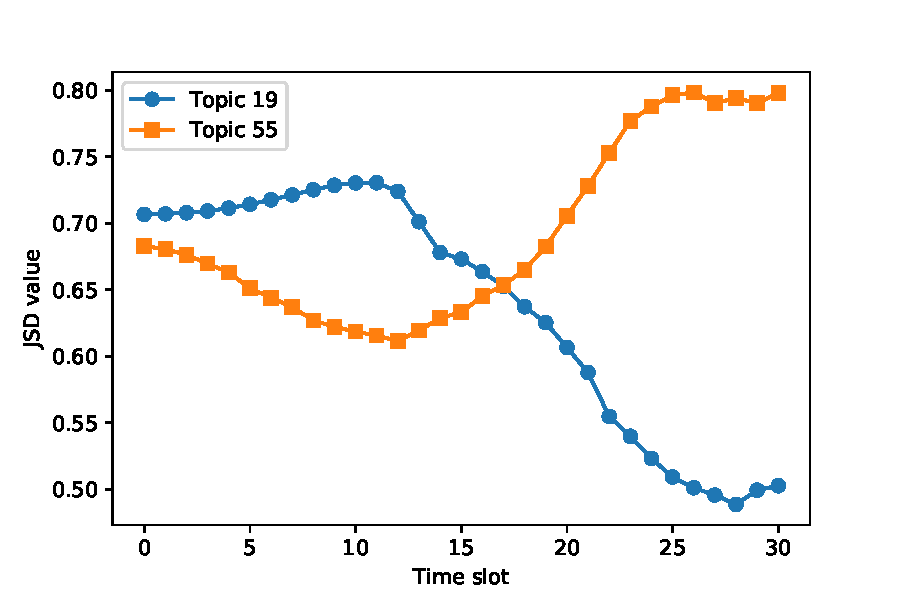
\includegraphics[scale=0.7]{JSgraph.pdf}
\tiny
\begin{tabular}{|p{7cm}|p{7cm}|}
\hline \bf LDA Topic 19 & \bf LDA Topic 55 \\ \hline

'rank', 'matrices', 'norm', 'tensor', 'entries', 'decomposition', 'columns', 'column', 'subspace', 'spectral', 'singular', 'completion', 'privacy', 'row', 'svd', 'trace', 'sparse', 'vectors', 'rows', 'private', 'product', 'diagonal', 'orthogonal', 'min', 'minimization', 'exact', 'factorization', 'differential', 'nuclear', 'symmetric', 'missing', 'entry', 'subspaces', 'recover', 'vec', 'tensors', 'arxiv', 'estimation', 'guarantees', 'noise', 'covariance', 'condition', 'power', 'projection', 'recovery', 'diag', 'norms', 'differentially', 'frobenius', 'k2f'
&
'noise', 'signal', 'components', 'component', 'filter', 'signals', 'source', 'filters', 'coefficients', 'mixture', 'noisy', 'sources', 'ica', 'separation', 'mixtures', 'filtering', 'variance', 'estimated', 'transform', 'blind', 'power', 'coding', 'wavelet', 'estimation', 'basis', 'snr', 'denoising', 'higher', 'invariant', 'gaussians', 'mixing', '1997', 'sensor', 'samples', 'unknown', 'orthogonal', 'fig', 'measurements', 'estimates', 'nonlinear', 'normalization', 'adaptive', 'overcomplete', 'equivalent', 'complex', 'correlated', 'elements', '2000', 'distributed', 'filtered'
\\ \hline

\end{tabular}
\caption{Models trained with the NeurIPS dataset with 60 topics for both DTM and LDA: Word distribution of DTM topic 0 at time slices T=0,5,10,15,20,25, and30 is shown in the first table. The last table shows the word distributions of LDA topics 19 and 55, respectively, and both curves in the graph are the JS similarity measure of DTM topic 0 with LDA topics 19 and 55. This is a graphical representation of two fragmented LDA topics related to one single DTM topic.}
\label{fig:fragmentation}
\end{center}
\end{figure*}

To extract DTM topic information from LDA, we use the inverse approach, which is to try to extract relevant information from LDA and, if the extracted information matches DTM's topics, then we can say that this technique is a good way to extract DTM's topics using LDA. For this comparison, we used different approaches.

\begin{itemize}
\item Overall correlation of LDA topics
\item Time-series topic correlation
\end{itemize}

Fragmentation means a single DTM topic contains two or more partial LDA topics. LDA topics that are related to a single DTM topic are similar in some aspect, so calculating the correlation among fragmented LDA topics is a good starting point. The correlation coefficient calculates the strength of the relationship between the relative movements of two variables, and the variables in this case are LDA topics that are calculated from the topics distribution $\theta_{dk}$. As DTM is time-dependent, it is better to also check the correlation of LDA topics in a series by categorizing documents with respect to time and then aggregating the correlation coefficient of each time slice.

Lastly, the time-series topic popularity, which is the second important information offered by DTM, can be extracted from the LDA topics. After calculating document-topic distribution $\theta_{dk}$. the documents are categorized with the same time-series information as used in DTM. Then, we calculate the estimated number of documents for each topic in a time series manner and construct a graph that is comparable to the DTM topics popularity information.